\documentclass[conference]{IEEEtran}

% -------------------------------------------------
% Packages
% -------------------------------------------------
\usepackage{graphicx}
\usepackage{booktabs}
\usepackage{amsmath}
\usepackage{siunitx}
\usepackage{placeins}
\usepackage{cite}
\usepackage{xurl}
\usepackage{multirow}
\usepackage{tabularx}
\usepackage{array}
\usepackage{tikz}
\usetikzlibrary{arrows.meta, positioning, shapes.geometric, calc}
\usepackage{listings}
\usepackage{xcolor}
\usepackage{fancyhdr}
\usepackage{float}

\lstset{
    basicstyle=\ttfamily\scriptsize,
    frame=single,
    breaklines=true,
    columns=fullflexible,
    numbers=left,
    numberstyle=\tiny,
    captionpos=b
}


% Optional: reduce excessive hyphenation
\hyphenation{Ardu-Pilot quad-copter Mission-Planner}

\begin{document}

% -------------------------------------------------
% Title and authors
% -------------------------------------------------
\title{EEOPS-D Practical Course Report: Design, Build and Testing of an
ArduPilot-Based Quadcopter}

\author{
\IEEEauthorblockN{
Mohammed Zaki Al-Chalabi,
Maksymillian Aniskiewicz-Chin,
Timothee Breabout,\\
Cameron Jones,
Oliver Montorio,
Nicholas Wright,
}
\IEEEauthorblockA{
Department of Engineering, Durham University\\
ENGI3301 / ENGI3371 Practical Course Assignment, June 2026
}
}

\maketitle
\thispagestyle{fancy}
\pagestyle{fancy}
\fancyhf{}              % Clear all header/footer fields
\fancyfoot[C]{\thepage} % Page number centred at the bottom
\renewcommand{\headrulewidth}{0pt}
\renewcommand{\footrulewidth}{0pt}

\tableofcontents
\thispagestyle{plain}

\section{Abstract}
The repeatable design, construction, and testing of an autonomous ArduPilot-based quadrotor provides a foundation for the development of UAV-based entrepreneurial solutions through appropriate hardware integration and software parameter tuning. This report details the assembly, configuration, calibration, and flight testing of the quadcopter, demonstrating a reproducible development methodology that can be adapted to a range of commercial applications. We validated a specific business case through integrating a first-person view (FPV) camera system onto the drone structure, enabling remote visual inspection of environments that are difficult for direct human access, such as disaster zones. Despite requiring extensive troubleshooting and iterative tuning due to component variability, the resulting flight-worthy platform demonstrates the viability of a repeatable UAV development process for application-specific business opportunities.


\section{Introduction}
The rapid growth of autonomous unmanned aerial vehicles (UAVs) has driven their adoption across commercial, industrial and emergency-response sectors. Although DJI dominates the consumer and prosumer UAV market through highly reliable, integrated platforms, their proprietary hardware and software ecosystems provide limited flexibility for application-specific hardware and software modification. Consequently, open-source flight control systems such as ArduPilot present an attractive alternative for developing custom UAV platforms tailored to unique operational requirements and entrepreneurial opportunities.

This report presents the design, construction and evaluation of an ArduPilot-based quadcopter developed as part of the EEOPS-D practical course. The project integrated mechanical design, 3D printing, electrical system assembly, flight-controller configuration, autonomous Lua scripting, camera-based inspection and computer-vision tracking to produce a flexible UAV platform capable of stable flight, live visual feedback and basic autonomous operation. By following a repeatable development methodology, the project demonstrates how open-source UAV platforms can be adapted to meet specific commercial requirements, with hazardous industrial inspection serving as a representative entrepreneurial application.
\maketitle

\section{System Design and Development [Z.A, T.B]}

\subsection*{UAV Avionics Hardware Integration and Pin Mapping}


The first stage of drone assembly required us to determine the correct wiring configuration of each external component and their interface into the central autopilot flight controller. We used the MicoAir743v2-AIO-45A [1] (hence referred to as the flight controller) developed by MicoAir, which is an “All-In-One” (AIO) flight controller as it includes an electronic speed control (ESC) on the same board (has the imbedded functionality to control and regulate motor speeds). The flight controller supports the firmware ArduPilot which enables the UAV to perform advanced autonomous flight capabilities such as waypoint navigation and failsafe management.  

\subsubsection*{Flight-Controller and Peripheral Wiring}

We implemented three external sensor devices to our quadrotor Unmanned Aerial Vehicle (UAV). The XR1 Nano Multi-Frequency ExpressLRS Receiver is the UAV’s radio control receiver. Its primary role is to communicate the instructions sent by the pilot’s transmitter and relay them to the flight controller. This transceiver supports the use of 900MHz transmission for longer potential range however we used the 2.4GHz frequency range for higher data rates and integration with our RC controller.  

The second device is the Matek M10Q-5883 (Compass/GPS) which contains both a u-blox M10-series GNSS receiver and a QMC5883L magnetometer (compass). The GNSS receiver simultaneously tracks multiple satellites constellations: GPS, GLONASS, Galileo and BeiDou, which gives accurate global positioning, ground speed and direction of travel. The magnetometer measures the Earth's magnetic field to determine the aircrafts heading relative to magnetic north. These enable advanced flight functions such as position hold and autonomous waypoint navigation, but require calibration to work in the first instance.  

The ESP32 Telemetry Module running Drone Bridge is responsible for providing a full wireless data link between the UAV and the computer ground station. Connected via a Universal Asynchronous Receiver/Transmitter (UART) interface, the module transmits MAVLink telemetry data including position, altitude, flight mode and battery health to the ArduPilot Mission Planner software. This enables real-time flight monitoring supporting the safety of our flight tests by giving live access to drone positioning and remaining battery. Having constant access to the battery voltage level in flight is important for the health of our battery (Tattu R-line 4s 850mAh 14.8V) as these rechargeable batteries are effectively dead if drained below 13V, which can happen very quickly when flying the drone.  

Each external device typically has a ground pin (GND), a live pin (5V), a transmit pin (TX) and a receive pin (RX). The ground and live wires allow the flow of current from the battery and flight control into the sensor, enabling them to draw power to carry out their intended function. TX and RX wires are one-way data lines which provide the pathway for instructions and data to travel between the flight controller and sensor which together form a serial communication interface (UART). In all cases, the 5V pin from the flight controller should connect to the 5V pin in the device, with the same direct connection for the GND pins. The TX on one device must connect to the RX on the other device as data must flow from the transmitter to the receiver (and vice versa with RX to TX). See Fig.~\ref{fig:fc-wiring-top} and Fig.~\ref{fig:fc-wiring-bottom}.

The Compass/GPS module additionally has Serial Data Line (SDL) and Serial Clock Line (SCL) pins which are used for an Inter-Integrated Circuit (I2C) communication interface, allowing the flight controller to talk to the onboard magnetometer. The SDA carries actual data between the flight controller, and the compass and the SDL provides a timing clock that synchronises when data is sent and read.  

% -------------------------------------------------
% Flight-controller wiring: top view
% -------------------------------------------------
\begin{figure}[htbp]
    \centering
    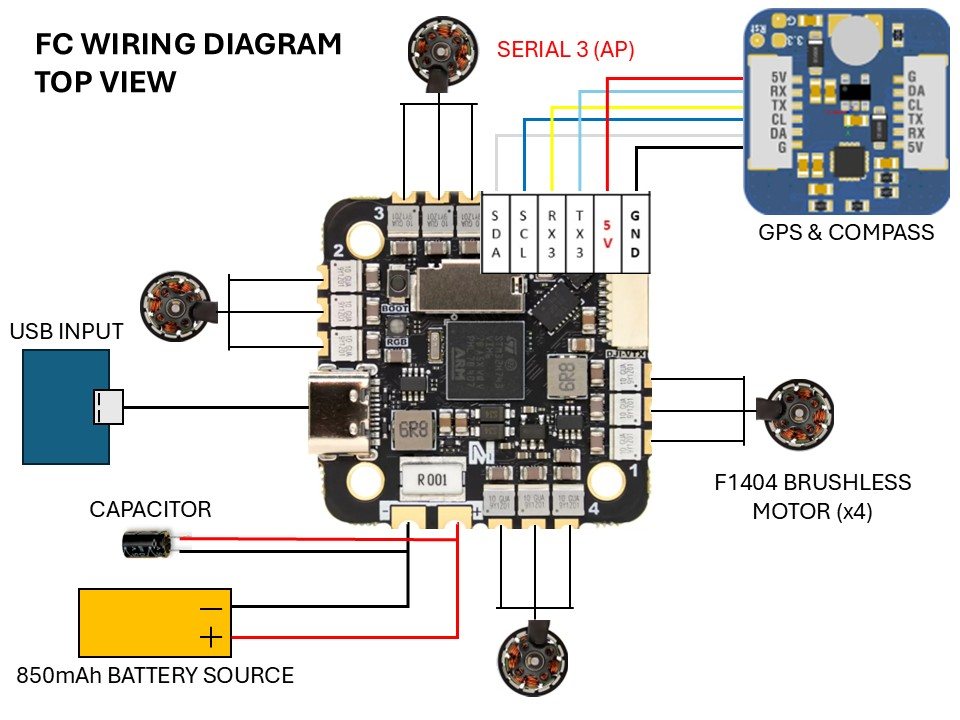
\includegraphics[width=\columnwidth]{Figures/Zaki1.JPG}
    \caption{Flight-controller wiring architecture viewed from above, including battery and capacitor connections, four F1404 brushless motors, USB interface, and the GPS/compass connection through Serial 3.}
    \label{fig:fc-wiring-top}
\end{figure}

% -------------------------------------------------
% Flight-controller wiring: bottom view
% -------------------------------------------------
\begin{figure}[h]
    \centering
    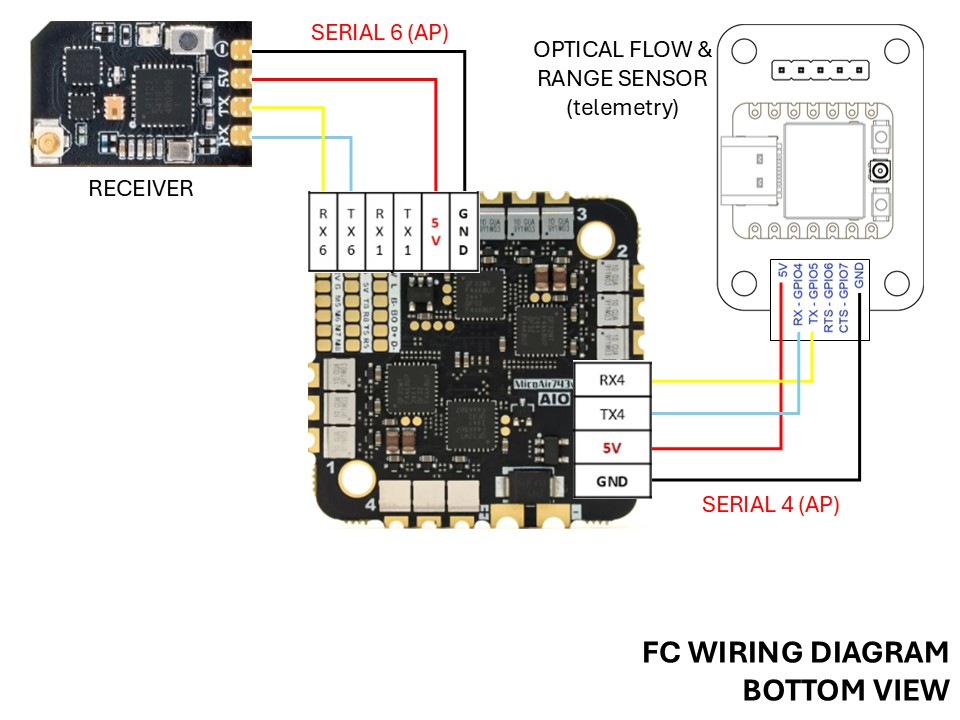
\includegraphics[width=\columnwidth]{Figures/Zaki2.JPG}
    \caption{Flight-controller wiring architecture viewed from below, including the ExpressLRS receiver connection through Serial 6 and the optical-flow and range-sensor connection through Serial 4.}
    \label{fig:fc-wiring-bottom}
\end{figure}

\subsubsection*{FPV Camera Integration}

Our UAV incorporates a miniature camera system to enable the wireless transmission of a live first-person view (FPV), looking out in the direction of forward motion of the drone. This added functionality allows for real-time visual feedback to the operator.

The exact name and model details for our camera system was unknown, which provided a unique troubleshooting process to determine the power required by the camera and the method of transmission. From market research, we identified similar models of small drone-based cameras operating at the \SI{5}{\volt} mark, and so we assumed our model would work similarly.

To assess our hypothesis and mitigate risk of component damage, we tested the camera independently using a variable voltage supply set at \SI{5}{\volt}. The camera was in-built with four output wires, red, black, yellow and white, and a radio signal transmitter. Red and black were assumed to be live and ground wires respectively, with the yellow and white wires used for transmission of the video stream in a wired connection. We tied off the white and yellow wires to nullify them in favour of the wireless radio transmission mechanism, which would allow the use to transmit the live camera feed to our ground station from long distances.

A DC--DC buck converter was required to step down the \SI{12}{\volt} outputted by the remaining port on the MicoAir flight controller, to the \SI{5}{\volt} required by the camera. The live \SI{12}{\volt} voltage output from the FC was soldered to the voltage input of the converter, with the voltage output pin on the converter being wired to the \SI{5}{\volt} input pin on the camera, as shown in Fig.~\ref{fig:fpv-power}. The ground wires were all connected together, and the \SI{5}{\volt} level on the converter was selected through soldering of the \SI{5}{\volt} resistor level. The camera was mounted onto the base of our drone using a 3d printed CAD gimble for stability.

\begin{figure}[htbp]
    \centering
    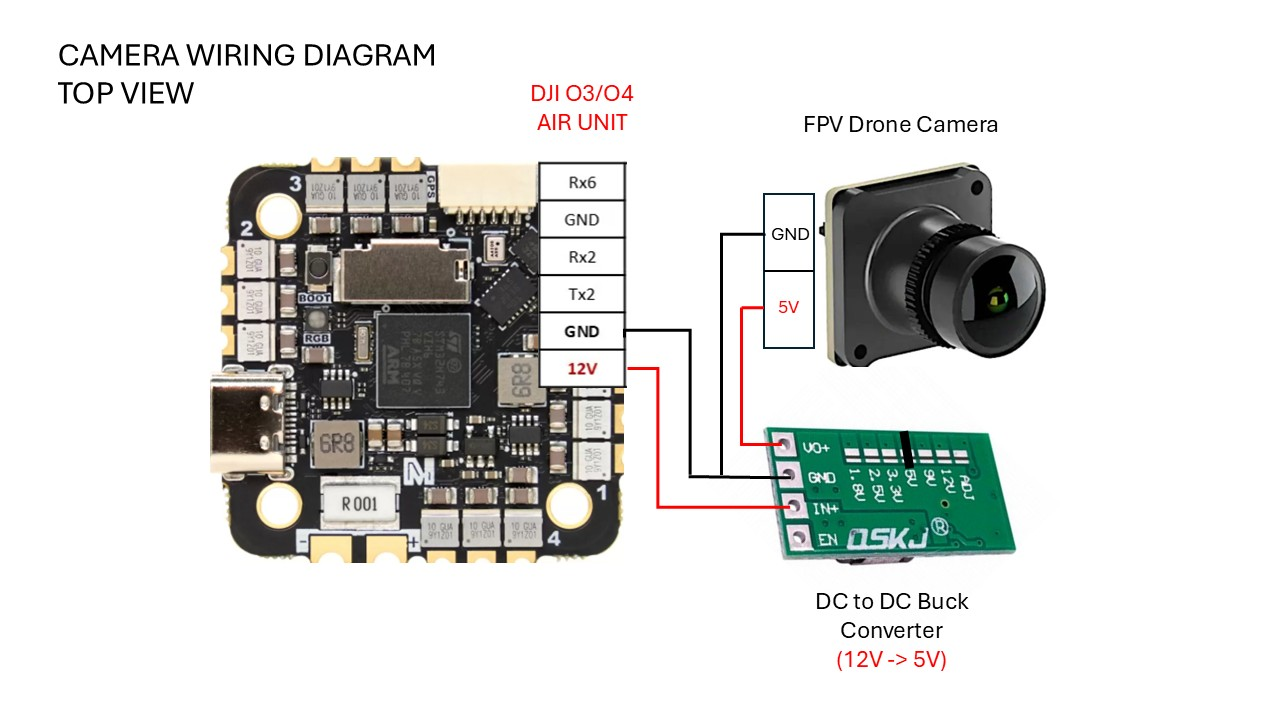
\includegraphics[width=\columnwidth]{Figures/Zaki3.JPG}
    \caption{FPV camera power architecture. The \SI{12}{\volt}
    flight-controller output is stepped down using a DC--DC buck
    converter to provide the regulated \SI{5}{\volt} supply required
    by the camera, with a common ground shared between all components.}
    \label{fig:fpv-power}
\end{figure}


\subsubsection*{Findings}
After connecting the live and ground wires to the \SI{5}{\volt} voltage supply, we validated that the camera was working correctly through verifying a stable current draw, along with a successful video output to our ground control laptops camera app. We found the camera's attached radio transmitter to be sending live its live feed at \SI{5737}{\mega\hertz} frequency to the receiver which was connected via USB to the laptop.

It was important to ensure wires were connected correctly. If two wires were swapped when connecting a device into the flight controller, there could be negative consequences. Swapping the RX, TX, SDA or SCA wires could prevent the devices from communicating, leading to no data or incorrect data readings. A more devastating error would be swapping 5V and GND wires, which could lead to short circuiting, overheating and can damage components. Reversing the polarity of the power by connecting the power backwards can destroy the microcontroller itself almost instantly after plugging in the battery. Excessive current draw, which could be caused by pin mismatches, will likely lead to the board heating up, and components emitting smoke. This was identified in the risk assessment as a major risk of the project.

% =================================================
\subsection*{Iterative Design of 3D-Printed Structural Components}

The iterative development of the 3D-printed structural frame was critical to this unmanned aerial vehicle (UAV) project. To achieve the sub-250g weight target whilst ensuring operational durability, Design for
Manufacture and Assembly (DFMA) principles were strictly applied. By methodically identifying vulnerabilities in early physical prototypes, such as assembly complexity, material yield strength, and geometric tolerances, subsequent SolidWorks CAD iterations successfully eliminated weak points, reduced fastener dependency, and optimised the drone for environmental hazards. The following sections detail the progression of the base plate, battery mount, battery mount lid, and camera gimbal.

% -------------------------------------------------
\subsubsection*{Iterative Design of the Base Plate}

The base plate provides a stable landing platform and protects the exposed wiring and SD card slot beneath the flight controller. Progressing through three iterations, the initial design featured a central housing with four short legs. Physical testing revealed this narrow footprint created a high centre of gravity, making the drone highly susceptible to tipping. To
address this, the second iteration significantly extended the legs to create a wider, thinner cross-shaped structure, incorporating an asymmetric arrow to indicate the drone's forward orientation. Whilst static stability and visual tracking improved, structural integrity was compromised; the thin legs flexed excessively, causing unpredictable bouncing, and ultimately snapped under the dynamic weight of landing.

Consequently, the third iteration abandoned individual legs for a large, continuous landing skid (Fig. 4). This complete geometric overhaul distributes impact forces effectively to prevent fractures. Furthermore, it provides increased propeller clearance for taking off in harsh conditions, such as long grass, and its ergonomic geometry permits safe hand-launching and
catching when ground landings are unviable.


\begin{figure}[htbh]
    \centering
    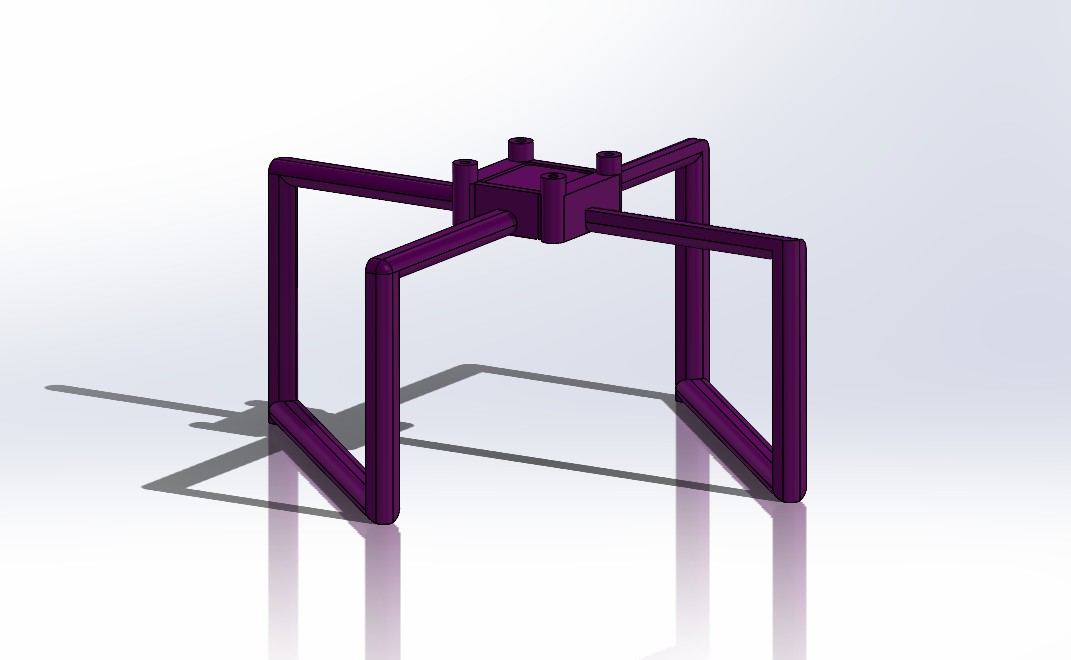
\includegraphics[width=\columnwidth]
    {Figures/BasePlate.png}
    \caption{Successive iterations of the 3D-printed base plate and
    landing structure.}
    \label{fig:base-plate-iterations}
\end{figure}

% -------------------------------------------------
\subsubsection*{Battery Mount Part Consolidation and Structural Reinforcement}

Subject to flight vibrations and rapid battery swaps, the battery mount required modifications to eliminate failure points and simplify assembly. The original three-pieces design relied on adhesive, which is vulnerable to fatigue and delamination in high-vibration environments. Furthermore, mating this assembly to the X-frame centre bracket required a highly
fiddly captive nut.

To resolve these issues, the mount was redesigned as a single, solid 3D-printed piece that integrated the top of the X-frame centre bracket directly into its structure (Fig. 5). This monolithic design eliminated both the
weak glued joints and the inefficient captive nut, drastically streamlining assembly whilst creating a rigid connection between the payload and the airframe. Finally, to address remaining concerns regarding lateral strength, a perpendicular cross-brace was added between the mount's vertical legs. This structural reinforcement prevents flexing or buckling under the lateral pressure of the battery during aggressive
flight manoeuvres or hard landings.

\begin{figure}[htbp]
    \centering
    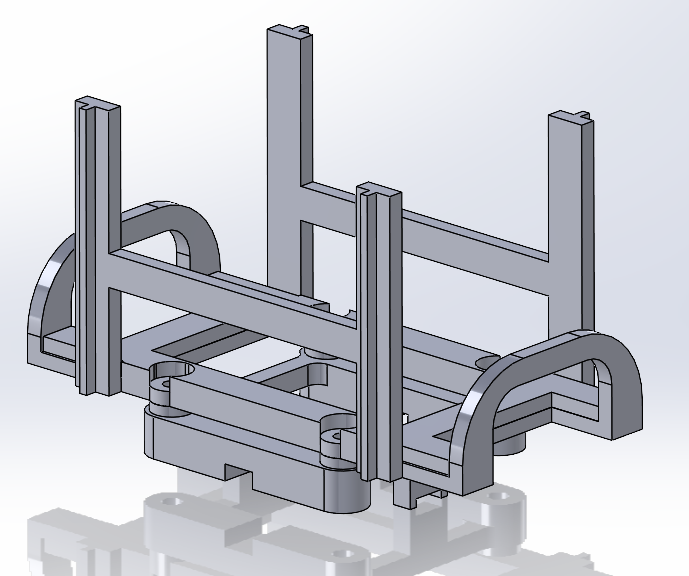
\includegraphics[width=0.65\columnwidth]
    {Figures/BatteryMount.png}
    \caption{Consolidated single-piece battery mount incorporating the
    X-frame centre bracket and lateral structural reinforcement.}
    \label{fig:battery-mount}
\end{figure}

% -------------------------------------------------
\subsubsection*{Battery Mount Lid}

The initial battery mount lid relied on simple caps secured to the vertical legs with superglue. Whilst this prevented battery ejection, it necessitated breaking the structural components apart to replace a
degraded battery or fix other parts. This destructive maintenance rendered the mount a single-use consumable, which was neither economically nor environmentally viable.

To combat this waste, a custom friction-fit iteration was developed (Fig. 6). The CAD geometry of the sliding caps was refined to perfectly mirror the external profile of the mount legs, creating a tight fit without adhesive.
Crucially, this system leverages the battery payload itself; the housed battery pushes outwards slightly against the vertical legs, creating internal friction that locks the slide-on lid securely in place. This
elegant mechanical solution ensures the payload remains secure under dynamic flight loads whilst allowing for easy, tool-less manual removal, keeping the components fully reusable and sustainable.

\begin{figure}[htbp]
    \centering
    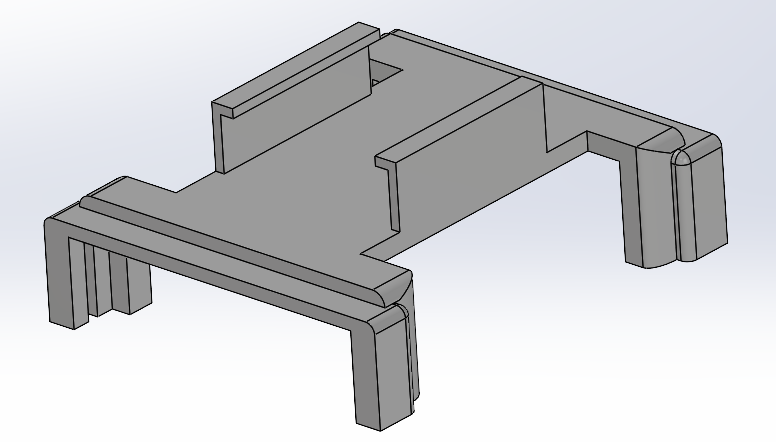
\includegraphics[width=0.65\columnwidth]
    {Figures/MountLid.png}
    \caption{Friction-fit battery mount lid designed for secure,
    adhesive-free and tool-less removal.}
    \label{fig:battery-mount-lid}
\end{figure}

% -------------------------------------------------
\subsubsection*{Single-Axis Friction Gimbal}

To provide adjustable visual feedback, a custom single-axis tilt gimbal was engineered to allow manual pitch articulation whilst maintaining a vibration-dampened airframe connection (Fig. 7). The assembly comprises three
3D-printed components: a base plate bolted to the frame, an outer U-shaped yoke, and a moving camera cradle with geometrically tailored walls and lips to securely retain the payload.

To adhere to weight constraints, the gimbal operates entirely without brushless motors or metal bearings, functioning instead as a mechanical friction hinge. Standard screws act as pivot shafts; by modulating their
clamping force, friction between the plastic components is controlled to hold the camera at any desired pitch angle. Aligning the pivot closely with the camera's centre of mass prevents sagging under its own weight.
Although lacking the absolute smoothness of an actively stabilised cinematic gimbal, this plastic-on-screw mechanism drastically reduces mass, part count, and mechanical complexity. By enabling manual tilt
adjustments for varied flight profiles, this highly printable design offers an elegant, lightweight  solution tailored specifically for FPV operations.

\begin{figure}[htbp]
    \centering
    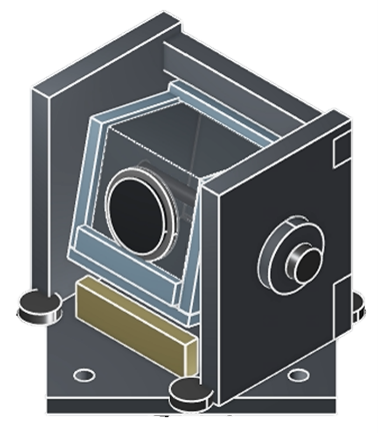
\includegraphics[width=0.65\columnwidth]
    {Figures/Gimbal.png}
    \caption{Single-axis friction gimbal comprising a frame-mounted base,
    U-shaped yoke and adjustable FPV camera cradle.}
    \label{fig:single-axis-gimbal}
\end{figure}

% =================================================
\subsection*{Mobile IFF Application}

As part of the multi-agent autonomy challenge, a mobile Identification Friend or Foe (IFF) application was developed to allow ground operators to rapidly distinguish between friendly and unknown drones in a shared airspace. The application runs on Android and operates entirely offline, requiring no network connectivity or specialist hardware beyond a standard smartphone.

% -------------------------------------------------
\subsubsection*{Design Rationale}

Traditional IFF systems rely on radio transponders and encrypted signal exchange, which are impractical at the scale of small consumer UAVs. The approach adopted here uses QR codes as a lightweight, low-cost identification mechanism. Each friendly drone is fitted with a printed QR code encoding a unique identifier. The operator points their device camera at any drone in the airspace; the application decodes the QR code in real time and classifies the drone as friendly or unknown, providing an immediate visual response overlaid on the live camera feed.

An initial concept explored on-device drone detection using a YOLOv8n TFLite machine learning model, which would have enabled identification without any physical marker on the drone. This was abandoned following
critical build failures caused by version incompatibilities in the native C++ layer, and the QR-based approach was adopted as a more reliable and
immediately deployable alternative. Machine learning-based detection remains a planned future development.

% -------------------------------------------------
\subsubsection*{Technical Implementation}

The application is built in React Native with Expo SDK 56. The core stack uses react-native-vision-camera for camera hardware access, configured at maximum frame rate to minimise motion blur on moving targets, and
vision-camera-code-scanner for per-frame QR decoding. When a code is detected, its value is checked against a locally stored list of approved identifiers. The result is rendered as a colour-coded bounding box directly onto the camera feed, green for friendly, red for unknown, alongside a HUD status indicator. A zoom slider (1×--5×), pinch-to-zoom gesture support, and a torch toggle were added following field testing to
improve scanning range and reliability.

The interface follows a military HUD aesthetic with a monospace green-on-black colour scheme, chosen for readability in outdoor conditions. The application installs independently on the operator's device and requires no configuration beyond granting camera permissions.

% Insert application screenshots here if available.
%
% \begin{figure}[!t]
%     \centering
%     \includegraphics[width=\columnwidth]{figures/iff-application.jpg}
%     \caption{Mobile IFF application interface showing QR-code detection,
%     target classification and the heads-up display.}
%     \label{fig:iff-application}
% \end{figure}

% -------------------------------------------------
\subsubsection*{Integration with the Broader System}

In the envisioned full system, GPS position data broadcast over drone tracking would narrow the camera's field of view to a drone's approximate screen location, enabling the QR scanner to lock on at significantly
greater range. This GPS-narrowed computer vision approach represents the next development phase, bridging the current manual aiming capability
with the longer-range autonomous identification required for full multi-agent operations. The system is also designed to scale, registering additional friendly drones requires only adding their identifier to the
approved list, with no rebuild of the application necessary.

% -------------------------------------------------


%=====================================================
\section{Autonomous Flight Development and Validation [C.J, M.C, Z.A]}

\subsection*{Lua-Based Autonomous Flight Development}
\label{sec:lua-development}

\subsubsection*{Simulation Environment and Initial Configuration}
The task at hand here was to program a Lua-based [4] autonomous flight sequence developed in ArduPilot, to command the quadcopter to take off, follow a closed square trajectory loop, returning to its
launch position and landing. Development and quantitative testing were initially completed using Mission Planner's software-in-the-loop (SITL) environment on a desktop computer. This enabled the control logic and safety behaviour to be tested without risking the physical aircraft.

The first attempt to launch SITL failed because several Cygwin runtime libraries required by \texttt{ArduCopter.exe}, including \texttt{cygiconv-2.dll} and \texttt{cygintl-8.dll}, were absent from the
active SITL directory. Re-downloading the SITL installation did not initially resolve the fault because Mission Planner was operating from a
OneDrive-redirected Documents directory, while the replacement libraries had been placed in the standard local Documents path. The active SITL working
directory was therefore identified and the required runtime libraries were placed beside \texttt{ArduCopter.exe}. This demonstrated that software-path management and external dependencies were significant potential failure sources independent of the flight-control logic.

Lua scripting was enabled by setting

\begin{equation}
    \texttt{SCR\_ENABLE}=1
\end{equation}

in the full parameter list and restarting the simulated flight controller.
Creation of the active \texttt{scripts} directory confirmed that scripting had
been enabled successfully.

Before autonomous navigation was attempted, a minimal diagnostic Lua script was installed with a successful outcome.

% =======================================================
% COMPACT LUA CONTROL-LOGIC SECTION

\subsubsection*{Autonomous Control Architecture}

The Lua controller was implemented as a non-blocking state machine rather than
as a delay-based command sequence. This allowed the script to monitor switch
state, vehicle mode, arming condition, position error and timeout faults while
progressing through the autonomous mission. The core mission logic is summarised
in Fig.~\ref{fig:compact-lua-flow}.

The mission was activated using \texttt{RC7\_OPTION = 300}, corresponding to
\texttt{Scripting1}. A deliberate LOW-to-HIGH switch transition was required
before the mission could start, preventing unintended activation immediately
after boot. Automatic arming was disabled, so the operator had to arm the
vehicle manually before the script could command take-off.

\begin{figure}[htbp]
\centering
\resizebox{\columnwidth}{!}{%
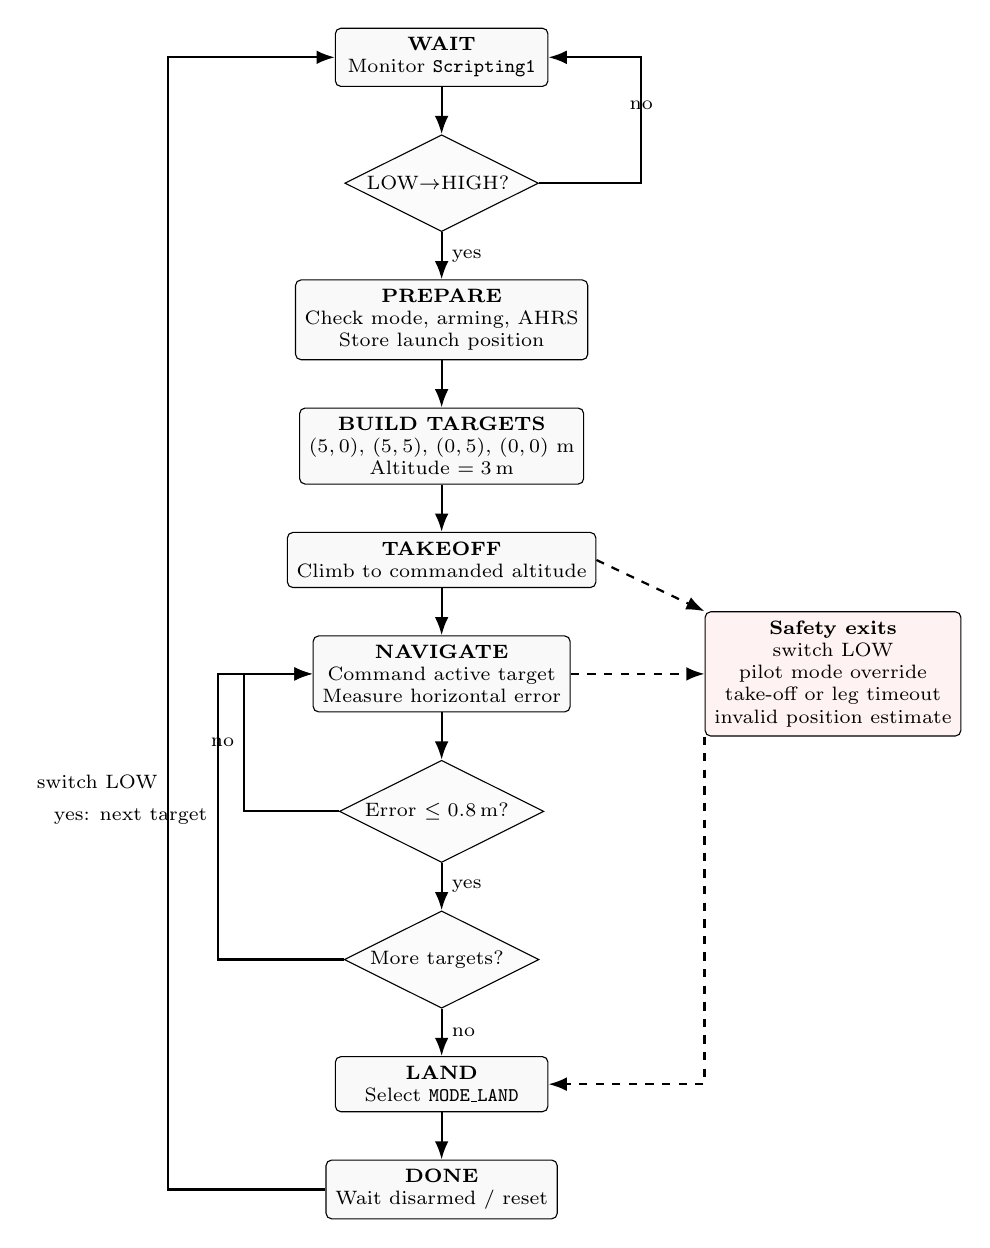
\begin{tikzpicture}[
    font=\scriptsize,
    node distance=6mm,
    block/.style={
        draw,
        rounded corners=2pt,
        align=center,
        minimum width=27mm,
        minimum height=7mm,
        fill=gray!5
    },
    decision/.style={
        draw,
        diamond,
        aspect=2.0,
        align=center,
        inner sep=1pt,
        fill=gray!3
    },
    safety/.style={
        draw,
        rounded corners=2pt,
        align=center,
        minimum width=31mm,
        minimum height=7mm,
        fill=red!5
    },
    arrow/.style={-Latex, thick},
    dashedarrow/.style={-Latex, thick, dashed}
]

% Main vertical state chain
\node[block] (wait) {
    \textbf{WAIT}\\
    Monitor \texttt{Scripting1}
};

\node[decision, below=of wait] (switch) {
    LOW$\rightarrow$HIGH?
};

\node[block, below=of switch] (checks) {
    \textbf{PREPARE}\\
    Check mode, arming, AHRS\\
    Store launch position
};

\node[block, below=of checks] (route) {
    \textbf{BUILD TARGETS}\\
    $(5,0)$, $(5,5)$, $(0,5)$, $(0,0)$ m\\
    Altitude $=3\,\mathrm{m}$
};

\node[block, below=of route] (takeoff) {
    \textbf{TAKEOFF}\\
    Climb to commanded altitude
};

\node[block, below=of takeoff] (nav) {
    \textbf{NAVIGATE}\\
    Command active target\\
    Measure horizontal error
};

\node[decision, below=of nav] (arrive) {
    Error $\leq 0.8\,\mathrm{m}$?
};

\node[decision, below=of arrive] (more) {
    More targets?
};

\node[block, below=of more] (land) {
    \textbf{LAND}\\
    Select \texttt{MODE\_LAND}
};

\node[block, below=of land] (done) {
    \textbf{DONE}\\
    Wait disarmed / reset
};

% Safety box to the right
\node[safety, right=17mm of nav] (safety) {
    \textbf{Safety exits}\\
    switch LOW\\
    pilot mode override\\
    take-off or leg timeout\\
    invalid position estimate
};

% Main arrows
\draw[arrow] (wait) -- (switch);
\draw[arrow] (switch) -- node[right] {yes} (checks);
\draw[arrow] (checks) -- (route);
\draw[arrow] (route) -- (takeoff);
\draw[arrow] (takeoff) -- (nav);
\draw[arrow] (nav) -- (arrive);
\draw[arrow] (arrive) -- node[right] {yes} (more);
\draw[arrow] (more) -- node[right] {no} (land);
\draw[arrow] (land) -- (done);

% Loops
\draw[arrow] (switch.east) -- ++(13mm,0) |- node[pos=0.25, above] {no} (wait.east);
\draw[arrow] (arrive.west) -- ++(-12mm,0) |- node[pos=0.25, left] {no} (nav.west);
\draw[arrow] (more.west) -- ++(-16mm,0) |- node[pos=0.25, left] {yes: next target} (nav.west);
\draw[arrow] (done.west) -- ++(-20mm,0) |- node[pos=0.18, left] {switch LOW} (wait.west);

% Safety arrows
\draw[dashedarrow] (takeoff.east) -- (safety.north west);
\draw[dashedarrow] (nav.east) -- (safety.west);
\draw[dashedarrow] (safety.south west) |- (land.east);

\end{tikzpicture}
}
\caption{Simplified state-machine representation of the Lua autonomous
closed-route script. Dashed transitions represent
abort, override and fault exits.}
\label{fig:compact-lua-flow}
\end{figure}

\subsubsection*{Route Definition}

The route was generated relative to the recorded launch position using four
local north-east offsets:
\begin{equation}
    (5,0),\quad (5,5),\quad (0,5),\quad (0,0)\ \mathrm{m}.
\end{equation}
The vehicle therefore followed a nominal $5\,\mathrm{m}\times5\,\mathrm{m}$
closed square at a commanded altitude of $3\,\mathrm{m}$. Each target was
accepted when the horizontal position error fell below the configured
$0.8\,\mathrm{m}$ acceptance radius. After the final target was accepted, the
script selected LAND mode.

\subsubsection*{Firmware Compatibility Correction}

A firmware-dependent Lua fault occurred during initial testing. The original
script used \texttt{set\_alt\_m()}, which was not available in the tested
ArduCopter firmware. This produced a scripting pre-arm error and prevented the
autonomous sequence from running. The altitude command was therefore rewritten
using firmware-compatible altitude handling, with altitude specified in
centimetres and the reference frame configured separately. After this change,
the pre-arm error disappeared and the full mission sequence executed
successfully. This showed that ArduPilot Lua scripts must be checked against the
specific firmware version used for testing rather than assumed to be portable
between releases.

\subsubsection*{Incremental Safety Validation}

The mission was tested incrementally before the complete route was attempted.
First, the vehicle was commanded to take off and the \texttt{Scripting1} switch
was moved LOW while airborne. The script responded by selecting LAND mode,
producing a controlled descent and disarm. Pilot authority was then tested by
manually changing the flight mode from GUIDED to BRAKE. The script detected the
external mode change and stopped issuing position targets, confirming that
manual or failsafe control retained priority over the Lua mission.

A reset procedure was also identified after landing. The vehicle could not be
re-armed while still in LAND mode, so the correct sequence was:
\begin{equation}
    \texttt{ LOW}
    \rightarrow
    \texttt{STABILIZE}
    \rightarrow
    \texttt{ARM}
    \rightarrow
    \texttt{ HIGH}.
\end{equation}
LOITER was initially considered for override testing, but in simulation it
caused descent because the virtual throttle input was not centred. BRAKE was
therefore used as the cleaner override mode because it held position without
requiring simulated throttle input.


\subsection*{Autonomous Flight Validation Results}
\label{sec:lua-results}

\subsubsection*{Functional Simulation Validation}

The corrected Lua script was first validated in SITL to confirm the autonomous sequence and safety exits before physical testing. Table~\ref{tab:sitl-functional-summary} summarises the functional checks.

\begin{table}[htbp]
\caption{Summary of SITL Functional Validation}
\label{tab:sitl-functional-summary}
\centering
\footnotesize
\renewcommand{\arraystretch}{1.05}
\begin{tabularx}{\columnwidth}{@{}lX@{}}
\toprule
\textbf{Validation item} & \textbf{Observed outcome} \\
\midrule
Mission sequence &
Take-off, four waypoint targets, return, LAND and disarm completed successfully. \\
Abort logic &
Moving \texttt{Scripting1} LOW terminated the mission and selected LAND. \\
Pilot override &
Changing from GUIDED to BRAKE stopped further scripted position commands. \\
\bottomrule
\end{tabularx}
\end{table}

These checks verified the script sequencing and control-authority hierarchy before the return-position accuracy was assessed quantitatively.

\subsubsection*{Quantitative Desktop SITL Results}

The script was extended to report the measured horizontal error at each target
and the final return error immediately before LAND was initiated. Six complete
desktop SITL trials were conducted using the same route definition and
waypoint-acceptance settings.

The recorded final return errors were

\begin{equation}
    0.61,\ 0.57,\ 0.64,\ 0.59,\ 0.63,\ 0.55\ \mathrm{m}.
    \label{return-errors}
\end{equation}

The mean return error was calculated as

\begin{equation}
    \bar{e}
    =
    0.598\,\mathrm{m},
\end{equation}

while the sample standard deviation was

\begin{equation}
    s_e
    =
    \sqrt{
    \frac{
    \sum_{i=1}^{n}
    (e_i-\bar{e})^2
    }{n-1}
    }
    =
    0.035\,\mathrm{m}.
\end{equation}

The simulated return performance is therefore reported as

\begin{equation}
    \bar{e}=0.598\pm0.035\,\mathrm{m},
\end{equation}

where the uncertainty represents one sample standard deviation rather than the standard error of the mean.

The mean final return error was $0.598\,\mathrm{m}$, equivalent to $12.0\%$ of one $5\,\mathrm{m}$ leg and $3.0\%$ of the $20\,\mathrm{m}$ route. However, this error is a final radial offset rather than an accumulated route error, so performance was assessed against the $0.8\,\mathrm{m}$ waypoint acceptance radius. All six trials satisfied this criterion. The low sample standard deviation indicates repeatable simulated behaviour. 

\subsubsection*{Illustrative Simulation Flight Path}

A separate Mission Planner installation was subsequently configured on a laptop. One  additional simulation run was performed to obtain a clear visual record of the autonomous route.

The laptop installation used ArduCopter V4.8.0-dev, build \texttt{0d6feaf5}, as shown in the Mission Planner title bar in Fig.~\ref{fig:simulation-path}. This run was completed after the quantitative desktop test campaign and was not included in the six-trial statistical dataset, hence the return error of $0.78\,\mathrm{m}$ not matching the errors in list \eqref{return-errors}. The distinction is necessary because different Mission Planner
installations can download different SITL firmware builds, and Lua API
availability can vary between ArduCopter versions.

The illustrative run completed the four-sided route, returned to the launch region within the $0.8\,\mathrm{m}$ waypoint-acceptance radius, entered LAND mode and disarmed.

\begin{figure}[htbp]
    \centering
    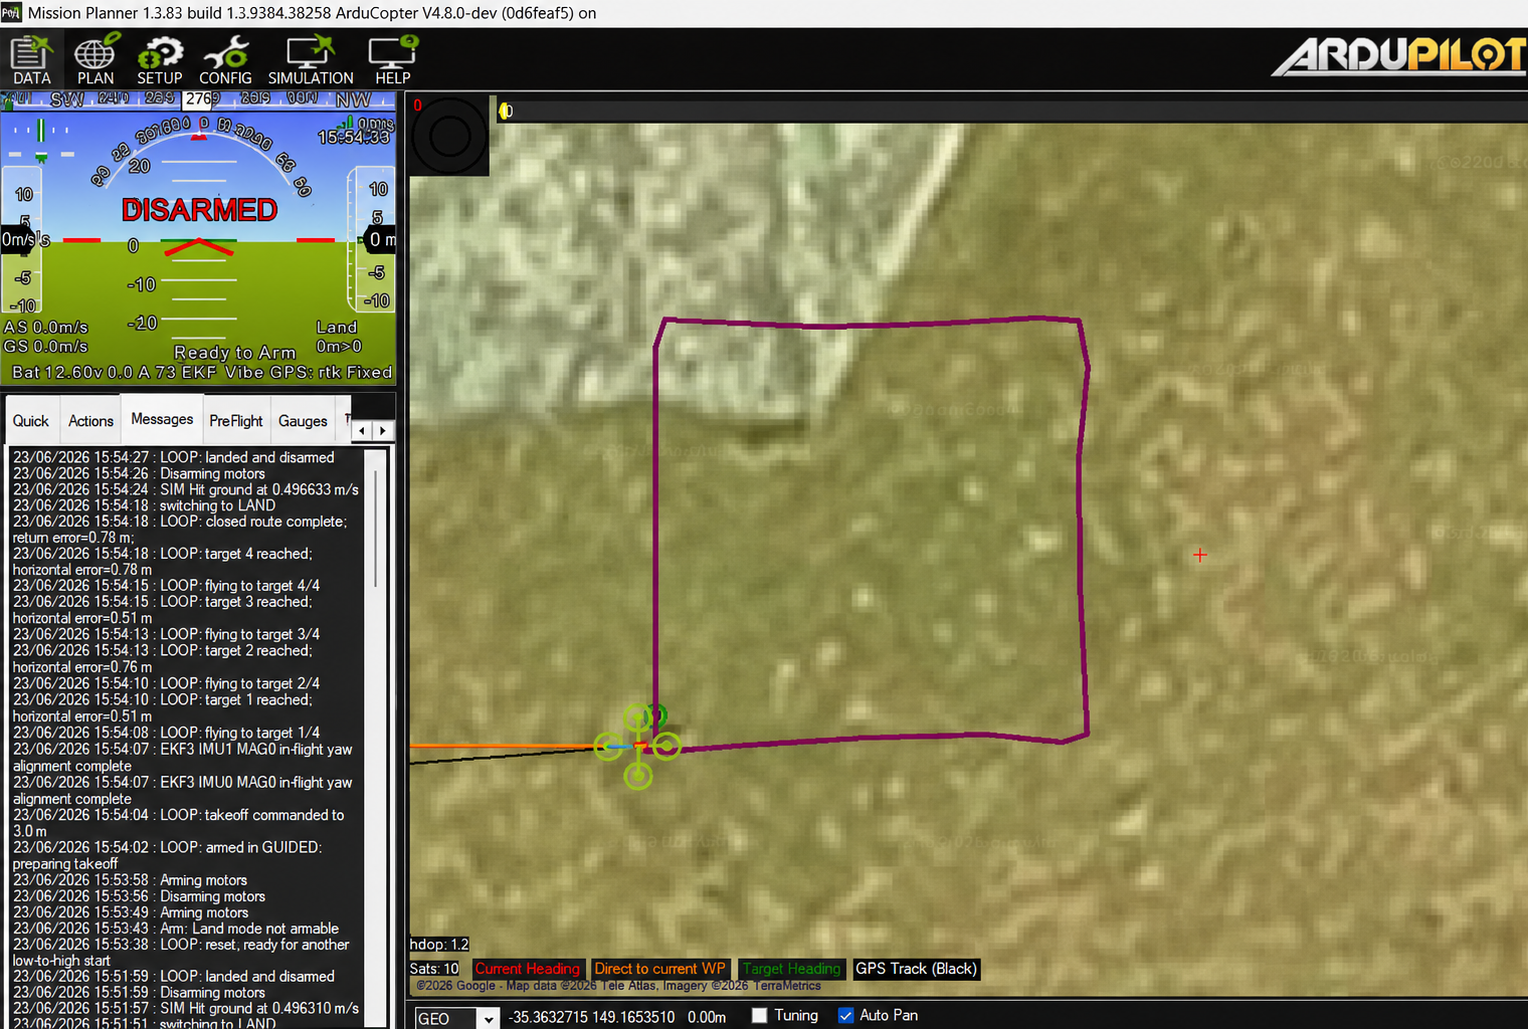
\includegraphics[width=0.9\columnwidth, trim={0 50 300 0}, clip]
    {Figures/LoopSimulation.png}
    \caption{Laptop SITL validation run showing the autonomous square-route trajectory.}
    \label{fig:simulation-path}
\end{figure}

\subsubsection*{Physical Flight Test}

The autonomous sequence was subsequently tested using the physical UAV. During
the flight, the aircraft was visibly displaced from the intended route by the
observed wind conditions. The onboard position controller then generated
corrective motion, returned the aircraft towards the commanded trajectory and
allowed the remaining waypoint sequence to continue.

The UAV subsequently returned to the launch region and completed the landing.
Figure~\ref{fig:physical-path} shows the recorded physical trajectory. The
large curved deviation in the flight trace corresponds to the period in which
the vehicle was displaced from the nominal square route before recovering. The
subsequent movement back towards the intended track indicates that the
position-control system attempted to reduce the displacement relative to the
active target rather than continuing along a permanently shifted path.

\begin{figure}[htbp]
    \centering
    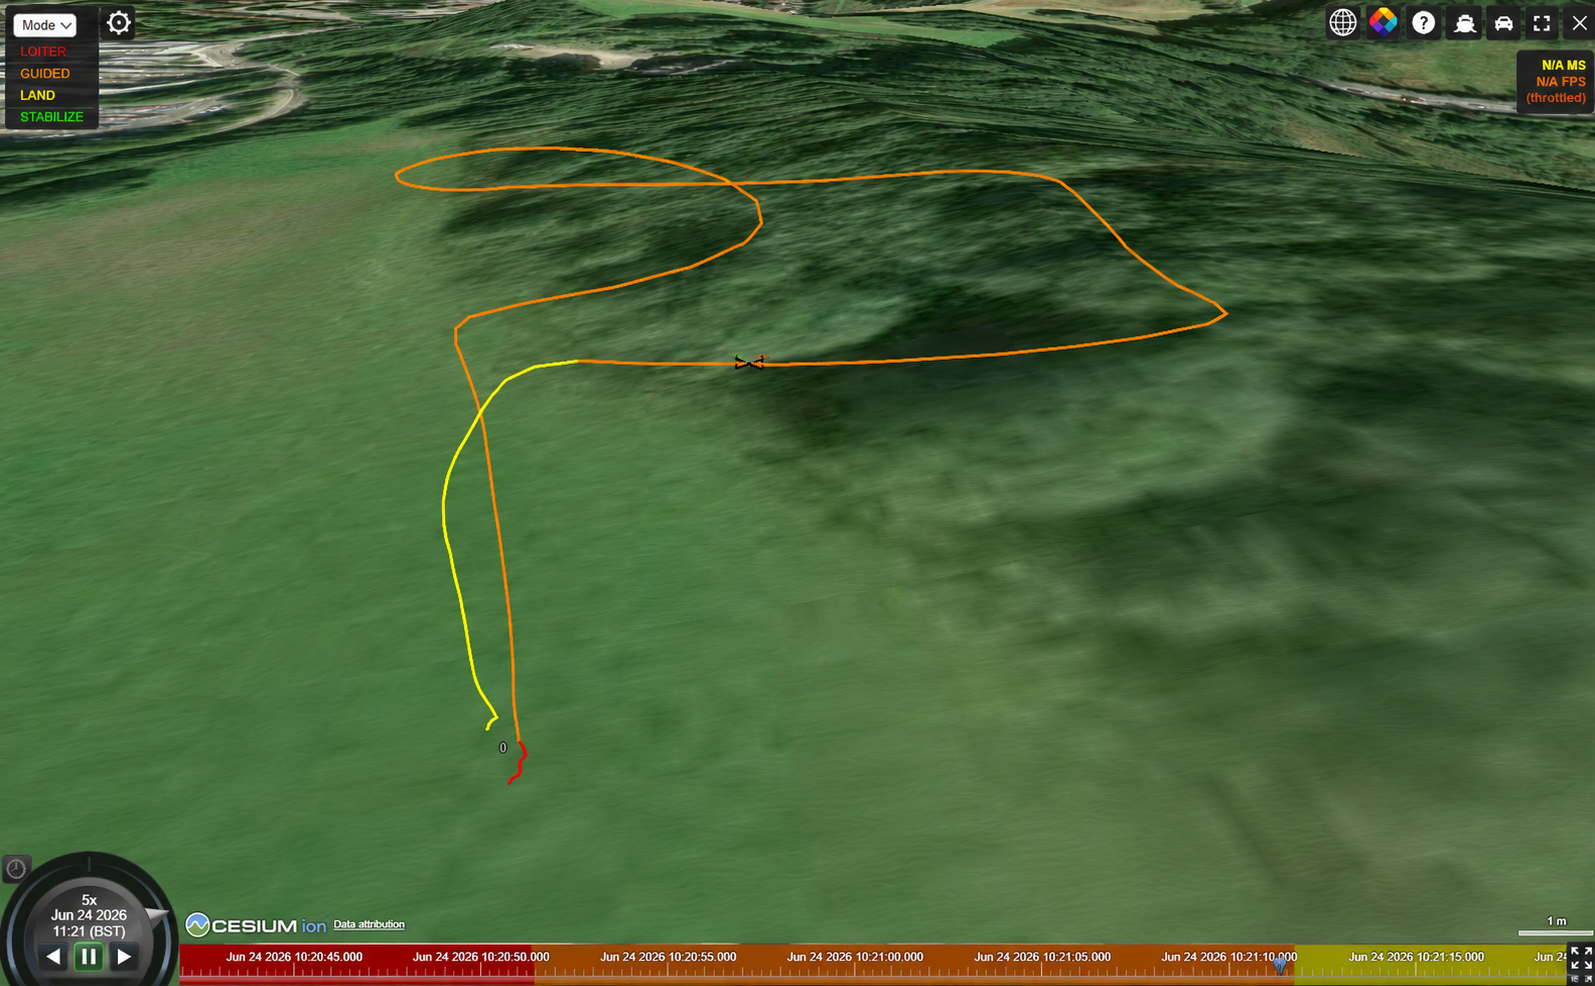
\includegraphics[width=0.9\columnwidth]
    {Figures/LoopReal.png}
    \caption{Physical flight trace showing wind displacement and subsequent route recovery.}
    \label{fig:physical-path}
\end{figure}

\subsubsection*{Troubleshooting and Validation Summary}

Two faults were significant during development. First, SITL failed to launch because required Cygwin runtime libraries were missing from the active Mission Planner SITL directory; this was resolved by identifying the correct OneDrive-redirected working directory and restoring the files beside \texttt{ArduCopter.exe}. Second, the initial Lua script produced a scripting pre-arm error because \texttt{set\_alt\_m()} was unsupported by the tested ArduCopter firmware. Replacing this with firmware-compatible altitude handling allowed the autonomous sequence to run. These faults were independent of the control logic but demonstrate the importance of dependency management and firmware-specific API checking.

\subsection*{Evaluation of Autonomous Flight Performance}
\label{sec:lua-discussion}

Across six desktop SITL trials, the aircraft completed the $20\,\mathrm{m}$ closed-square route with a mean final return error of $0.598\pm0.035\,\mathrm{m}$. Individual errors ranged from $0.55$ to $0.64\,\mathrm{m}$, giving a range of $0.09\,\mathrm{m}$ and a coefficient of variation of $5.8\%$. The low spread indicates repeatable simulated behaviour, but the approximately $0.60\,\mathrm{m}$ offset represents
moderate rather than high absolute positional accuracy. Since this is a final radial return error rather than an accumulated route error, performance is best assessed against the configured $0.8\,\mathrm{m}$ waypoint acceptance radius, which all trials satisfied.

The measured return error was partly determined by the acceptance logic. The script declared the final target reached as soon as the vehicle entered the $0.8\,\mathrm{m}$ acceptance region, without requiring low horizontal velocity or a dwell time near the launch coordinate. This explains why the separate illustrative laptop SITL run in Fig.~\ref{fig:simulation-path} could accept the final target with a reported $0.78\,\mathrm{m}$ return error. A more stringent
implementation would combine a smaller acceptance radius with a velocity or dwell-time condition, although an excessively small threshold could prevent reliable progression under noisy GNSS measurements.

The physical flight demonstrated mission completion under real disturbance rather than precise path tracking. The vehicle was visibly displaced from the nominal square route by wind, but the position controller reduced the error,
returned towards the active waypoint sequence and completed the landing within the observed launch region. This confirms disturbance recovery and pilot-safe mission execution, but it does not prove that the physical vehicle achieved the same positional accuracy as SITL. The screenshots are qualitative only because the simulated and physical traces use different viewpoints, scales and visualisation systems. A stronger validation would export flight-log positions into a common local north-east coordinate system and compare cross-track error, return error and recovery time across repeated physical trials.

% -------------------------------------------------
\section{Practical Assembly and Integration [ALL]}

\subsection*{Practical Design, Assembly and Calibration Process and Challenges }

\subsubsection*{Design Planning and CAD Preparation}

The practical build process began by planning how the main drone components would be connected and positioned. Before assembly, a wiring diagram was produced to map out the connections between the flight controller, receiver, GPS/compass module, motors, battery and other electrical components (Section I).

The physical design process then moved into CAD preparation and 3D printing. Existing CAD files were downloaded and reviewed, with the relevant components selected for the initial build. The carbon fibre beams were not printed but were used as structural members between the central frame and the motors. During assembly, callipers were used to set the spacing between the centre of the frame and each motor mount. Equal motor spacing was important because uneven arm lengths would shift the thrust positions relative to the centre of mass, making the drone more difficult to control and tune.

\subsubsection*{Mechanical Assembly and Electrical Integration}
Once the printed components and beams were prepared, the drone was mechanically assembled. The central frame was built first, followed by the installation of the motor mounts, propeller guards and battery holder. The flight controller was then mounted securely within the frame, and the wiring was completed using the wiring diagram as a guide. Care was taken to connect the receiver, compass and motor outputs correctly, as incorrect wiring could prevent the drone from communicating properly with ArduPilot or responding correctly during calibration.


\subsubsection*{ArduPilot Configuration}

After the hardware assembly was complete, the focus shifted to understanding and configuring the ArduPilot software through Mission Planner [2]. This stage involved working through the main setup procedures, including initial parameter setup, accelerometer calibration, compass calibration, radio calibration, motor testing, flight mode setup and failsafe configuration. The flight modes were set up, including Stabilize, Loiter and Land. Battery and safety-related parameters were also configured as part of the setup process, with the specific parameter \texttt{MOT\_BAT\_CURR\_MAX} being identified as crucial to performance saftey. This limits the current draw per motor, which we set to 5 to keep maximum current draw from all motors under 20A. If left unchecked, it is possible the flight controller may supply much more current than required and this can lead to excess heat being produced and the fuse being set off. 


\subsubsection*{Radio-Control Troubleshooting}

One of the first major challenges was getting the radio controller to communicate correctly with ArduPilot Mission Planner showed that an RC input was being detected, but the individual control channels were not moving, meaning that the transmitter inputs could not yet be used for calibration. The issue was first investigated by checking the receiver and transmitter settings, along with the ArduPilot parameters related to the RX/TX communication link. The RX and TX cable positions were also swapped to test whether the problem was caused by incorrect wiring. When this did not solve the issue, the receiver was replaced, but the same fault remained, suggesting that the receiver hardware was not the cause.

Because the system used an ExpressLRS receiver, the transmitter and receiver setup had to match the CRSF-based RC input configuration expected by ArduPilot. The fault was eventually traced to the transmitter being set to MAVLink mode rather than the normal RC control mode. This explained why ArduPilot could detect an RC connection, but the control channel values were not changing in Mission Planner. Once the transmitter mode was corrected, the radio channels responded properly, and the radio calibration process could be completed.



\subsubsection*{Compass Calibration Troubleshooting}

The next significant challenge was compass calibration. Initially, no compass was shown on the compass calibration screen despite the GPS/compass module being connected. The GPS/compass connection was checked against the required pin order, including GND, SDA, SCL, TX/RX and VCC connections between the Mateksys M10Q-5883 and the flight controller. Compass-related parameters were also reviewed, but the compass was still not detected. The issue was eventually found to be a bent pin in the connector where the compass plugged into the flight controller. After this physical fault was identified and corrected, the compass was detected correctly, and the calibration could be completed. This demonstrated the importance of checking both software settings and physical connector integrity during troubleshooting.



\subsubsection*{Motor Configuration and Testing}

Motor testing was then carried out to check that each motor was assigned correctly and spinning in the correct direction. The motor setup used the digital DShot ESC configuration supported by the MicoAir743-AIO-45A. This was useful because DShot provides digital communication between the flight controller and ESCs and does not require the same manual ESC calibration process as traditional PWM ESCs. Where required, motor direction was adjusted through the software rather than by physically changing the wiring. The motors were then checked again to confirm that they responded correctly before the drone was prepared for powered testing.



\subsubsection*{Power-System Failure and Flight-Controller Replacement}

Before the battery was used, it was verified through a staff-supervised smoke test to check that it was safe to connect. During later powered testing, a fault occurred when the battery was connected: a burning smell was noticed, the flight controller became hot and the board stopped functioning. This was understood to be due to the fuse built into the flight controller being damaged. As a result, the flight controller had to be replaced. Although this delayed the build process, it also highlighted the importance of confirming all power and current protection settings before live testing.

After receiving a replacement flight controller, the drone was disassembled and rebuilt using the existing usable components. The wiring, mounting and setup procedures were then repeated, including the calibrations and motor checks. This required much of the configuration work to be completed again, but the previous troubleshooting experience made the second setup process much more efficient. Once the rebuild and recalibration were complete, the drone was prepared for an initial take-off test.


\subsubsection*{Final Flight Validation}

The final assembled drone was able to take off and maintain a stable hover. This confirmed that the main practical assembly, wiring, calibration and setup processes had been completed successfully. The successful hover showed that the drone had reached a functional state after the build and calibration process.

\subsection*{Ground-Based Computer Vision Tracking and IFF System}
A ground-station computer vision system was developed to detect, track and identify the UAV from a live video feed. The system was designed as a lightweight Identification Friend or Foe (IFF) prototype, using visual information. The final implementation used Python, OpenCV and \texttt{opencv-contrib-python} this combined motion detection, red-marker segmentation, QR-code decoding and object tracking in one live loop.

The first prototype was developed in Lua and used OpenCV for basic drone detection. This version used background subtraction to detect changing regions between frames. The resulting binary motion mask was thresholded, cleaned using morphological opening and dilation, and passed through contour detection to generate bounding boxes around moving objects. This confirmed that drone movement could be detected from video, but it also showed a major limitation: the algorithm detected pixel changes rather than the UAV itself, therefore moving trees, people and shadows were also detected as possible drone motion (Fig. 11).

As the task expanded to include tracking and QR-based identification, the system was transferred from Lua to Python. This was justified because Python provided stronger OpenCV support, direct access to \texttt{cv2.QRCodeDetector()} and compatibility with \texttt{opencv-contrib-python} tracking algorithms. KCF and CSRT trackers were tested. CSRT was generally more accurate but slower, while KCF was selected for live operation because it gave lower latency. The tracker follows a selected or identified bounding box between frames, reducing the need to re-detect the drone from scratch in every frame. Manual selection using a key press was kept as a fall back if automatic tracking failed..

A red marker detection routine was added to improve visibility of the drone against cluttered backgrounds. The frame was converted from BGR to HSV colour space and red pixels were isolated using two hue ranges, since red wraps around the HSV hue axis. The red mask was then cleaned and converted into contour candidates. Early testing showed that static red objects, such as brick walls, could fool the tracker. To fix this, the reacquisition logic used a weighted scoring system, shown in Listing~\ref{lst:reacquisition_scoring}. Moving red candidates were given the highest score, ordinary moving candidates were still considered, and static red objects were heavily penalised. Candidates far from the previous drone position were also penalised, reducing the chance of the tracker jumping to unrelated background objects.



\begin{minipage}{\columnwidth}
\begin{lstlisting}[language=Python, caption={Simplified candidate scoring used for tracker reacquisition.}, label={lst:reacquisition_scoring}]
for candidate in all_candidates:
score = 0

if candidate.type == "red_moving":
    score += 600
elif candidate.type == "motion":
    score += 300
elif candidate.type == "red_static":
    score -= 1200

score += 0.3 * candidate.area

if last_position is not None:
    d = distance(candidate.centre, last_position)
    score -= 3 * d

    if d > search_radius:
        score -= 1500

select highest scoring candidate
restart tracker around selected candidate
\end{lstlisting}
\end{minipage}




QR-code decoding was then added for IFF classification. Each approved UAV was assigned a printed QR code containing a unique identifier, such as \texttt{FRIENDLY\_DRONE\_1}. The decoded text was compared against a list of approved identifiers; a match labelled the drone as friendly, while any other decoded identifier was labelled unknown. QR decoding was used mainly for identification rather than continuous tracking, because the code becomes increasingly difficult to read, the further away and faster the drone if flying. Therefore, to get the best reading, the program scanned both the full video frame and a zoomed-in crop around the tracker box, saving the ID once it was read.

Live video was provided using an Android IP Webcam stream over USB tethering. Direct use of \texttt{cv2.VideoCapture} caused latency because frames buffered faster than they could be processed. A threaded capture class was therefore implemented to continuously read frames in the background and store only the newest frame. The main loop then processed the latest available image instead of delayed buffered frames. Further optimisation was achieved by reducing processing resolution, using KCF for live tracking, reducing QR scan frequency and disabling debug windows by default. The display image was enlarged separately using aspect-ratio padding this improved visibility without increasing the internal processing load.

\begin{figure}[h]
\centering
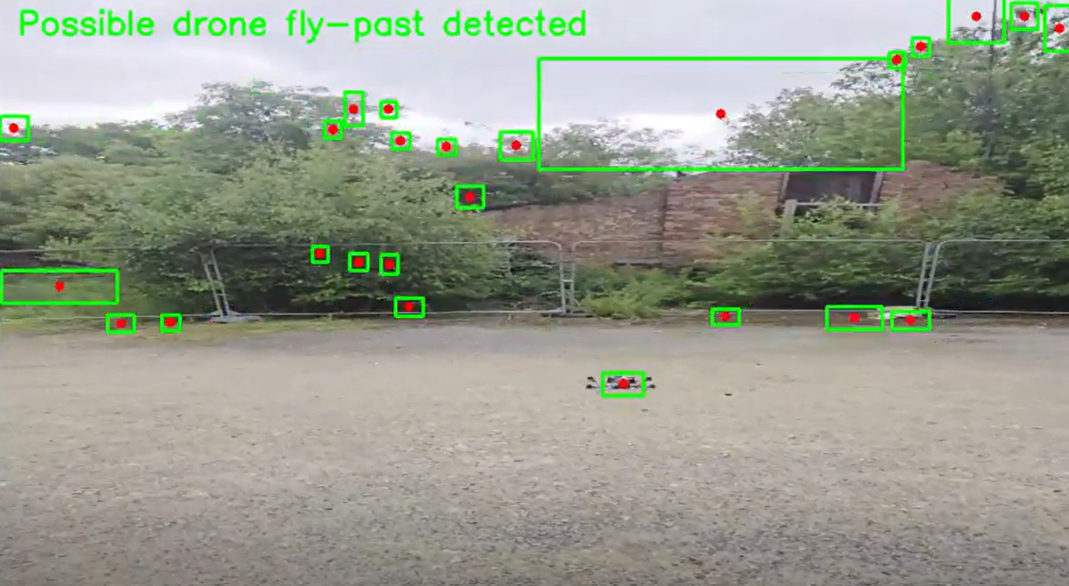
\includegraphics[width=0.95\columnwidth]{Figures/falsepositivesreport.png}
\caption{Initial motion-detection output showing false-positive detections from background movement and image noise. Although the UAV could be detected, trees, shadows and other moving regions were also identified as possible drone candidates.}
\label{fig}
\end{figure}

\subsubsection*{Testing, Troubleshooting and Critical Evaluation}
Testing proved that the final prototype could process a live camera feed, track a selected UAV, display a trajectory history and classify QR-coded targets as friendly or unknown (Fig. 12). The software developed through several troubleshooting stages. The Lua prototype proved the motion-detection concept but was limited by library support, leading the Python migration. Early Python motion detection produced many false positives, so object tracking was added. Tracker drift then occurred near cluttered backgrounds, leading to red-marker tracking and then the movement-prioritised red tracking logic. Live-feed lag was reduced using threaded capture, lower processing resolution and less frequent QR scanning.

The system remained most reliable when the drone was close to the camera, clearly visible and moving against a simple background. Performance reduced when the UAV became small, blurred or passed in front of trees, gravel or brick walls. QR detection was also limited during flight because the printed code had to remain large, flat and sharp enough to decode. Therefore, the QR code is best used to identify the drone before or during take-off, while the tracker and red marker are used to maintain the track afterwards (Fig. 13).

The main drawback is that the system uses traditional computer vision, meaning it cannot actually identify a drone by sight. Instead, it tracks basic features like motion, colour and shapes, which makes it sensitive to bad lighting, motion blur and camera resolution. However, this approach fit the goals as it was easy to understand and fit the timeframe given. Future improvements could be made by using ArUco markers instead of QR codes, better camera lens, or by using a YOLO machine learning model for better drone recognition.

\begin{figure}[h]
    \centering
    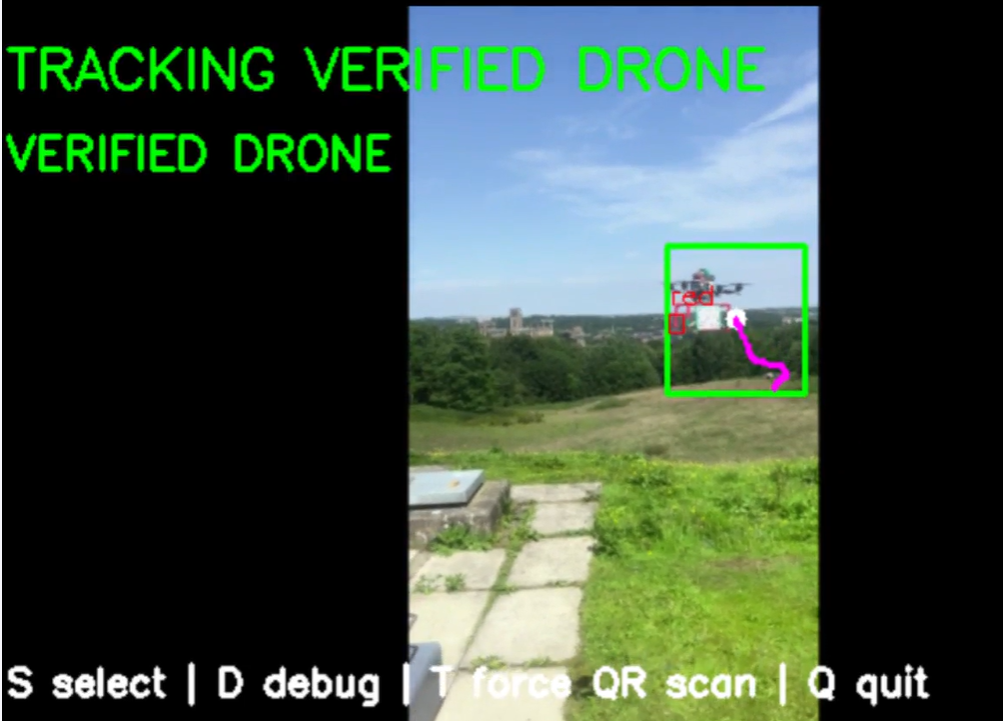
\includegraphics[width=0.85\columnwidth]{Figures/qrcodedetectedreport.png}
    \caption{Successful IFF demonstration showing the UAV classified as verified and tracked using a bounding box and trajectory history. The output combines QR-based identification with OpenCV object tracking.}
    \label{fig:verified_tracking}
\end{figure}

\begin{figure}[H]
    \centering
    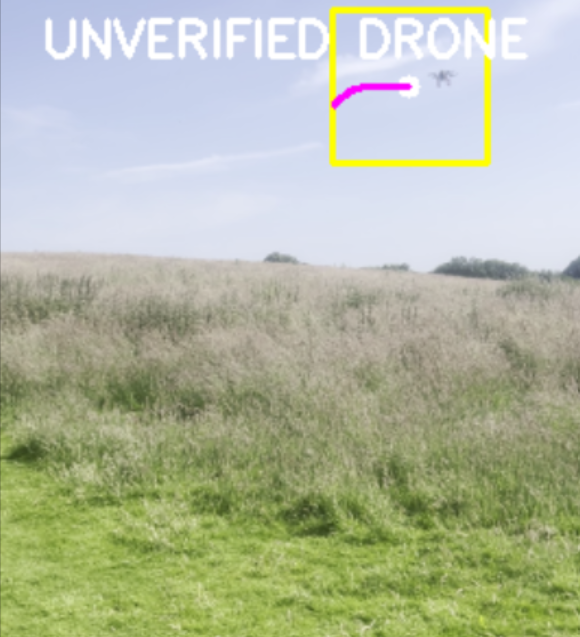
\includegraphics[width=0.85\columnwidth]{Figures/unverifieddrone.png}
    \caption{Long-range tracking output where the UAV remains within the tracking box, but QR-code identification is unreliable because the target is small, distant and partially blurred. This demonstrates why QR decoding was used mainly for initial identification, while object tracking maintained the UAV position afterwards.}
    \label{fig:unverified_tracking}
\end{figure}


\section{Business Case: Autonomous Visual Inspection of Hazardous Industrial Environments [T.B, N.W]}

\subsection*{Introduction}

In any industrial facility such as power stations, chemical processing plants, manufacturing facilities or large warehouses it is an essential requirement to regularly inspect any possible liability or risk around the facility in order to ensure that everything is operating safely but also to identify any potential future faults before they develop into serious failures. Nowadays a big majority of these inspections involve accessing elevated structures, confined spaces or any other potentially hazardous environments, therefore exposing workers to significant safety risks and increasing operational costs.

Traditionally, inspection methods require trained personnel who are able to use complex specialist access equipment and also cause temporary shutdowns of any operation during the time of the inspection. All these factors increase not only maintenance costs but also definitely reduce overall productivity. The companies managing these facilities are therefore at a stalemate between prioritise worker safety and making sure they keep high operational efficiency. There is therefore an increasing demand for a solution to this problem. This can be resolved with the use of our design: the drone  offers the possibility to remotely inspect hazardous areas while gathering accurate information without requiring personnel to enter.

Our objective with this project is to investigate how a lightweight autonomous drone can offer a low-cost alternative to the risky conventional inspection methods by taking advantage of the remote visual monitoring capabilities it offers.

\subsection*{Proposed Solution}

The proposed solution to this industry problem is a lightweight autonomous inspection drone which is capable of providing real-time live visual feedback from any hazardous or inaccessible locations. The system combines autonomous navigation, telemetry monitoring and most of all live video transmission. All these technicalities create a perfect package for a simple to build, cheap and easy to control drone well suited for remote inspection operations.

The drone can be deployed quickly and can even be deployed from the users hand. This allows for a quick setup before sending the drone towards areas of interest whilst continuously transmitting live imagery to its operators that are located at a safe distance. The engineers can then assess equipment conditions without requiring immediate any physical access to the inspection area with the possibility of keeping the live footage for further inspection at a later time.

The compact size of the drone and its simplistic base design enables it to be operated in confined environments while maintaining a low overall system cost compared to most commercial industrial inspection platforms available on the market right now.

\subsection*{Camera System Integration}

The primary enhancement that the team implemented to this project was the integration of an onboard camera system. This addition turns the drone from a simple navigation and flight platform into a practical inspection tool that is capable of collecting valuable operational data.

The camera gives a first-person view (FPV) of the drone’s surroundings and allows the operator to “see through the drone”. In other words it allows him to inspect the infrastructure remotely and can then identify potential defects. The real-time video transmission enables an immediate and rapid assessment of any location (Fig. 14).

The camera system also improves the general situational awareness of the pilot during flight operations as it can be used to verify navigation routes, monitor obstacles and inspect areas that would otherwise be inaccessible from ground level (Fig. 15).

This enhancement seemed evident since it directly supports the project’s main objective of reducing the need for personnel to enter hazardous environments while maintaining the same high standard level of inspection effectiveness.

\subsection*{Stakeholders}

Several stakeholders would benefit from the implementation of this technology.

First of all industrial facility operators would greatly benefit from reduced inspection costs and improved operational efficiency since the systems would require a much shorter shutdown time for inspection. In addition, the health and safety teams would gain from reduced worker exposure to hazardous environments as they would remain far from any dangerous sites. And finally maintenance engineers would have a quick and easy method to access real-time visual data without requiring physical access to inspection locations.

This system would however require the drone operator to be trained and qualified to flight the drone. This could therefore provide opportunities for any specialist drone service providers who could offer inspection services to industries that do not possess in-house drone capabilities.

This whole process would also satisfy any regulatory and safety organisations and company insurances as the infrastructure would benefit from an improved inspection record and more frequent monitoring of any critical infrastructures.

\subsection*{Economic Benefits}

The use of an autonomous inspection drone has the potential to greatly reduce the usual costs that are associated with traditional inspection methods.

Conventionally, inspections often require multiple personnel with equipment to access these remote areas and also temporary disruption of operations in order to mitigate any possible risk. By contrast, a drone-based inspection would be deployed rapidly and require little to no  preemptive setup.


\begin{itemize}

    \item A reduction of labour costs.

    \item A reduction of equipment hire costs.

    \item Faster inspection completion times.

    \item Reduced operational downtime.

    \item Earlier identification of any possible infrastructure defects.

\end{itemize}

The relatively low manufacturing cost of the drone is a major factor in its attractiveness for small and medium-sized enterprises that may be unable to justify investment in expensive and space consuming commercial inspection systems.

\subsection*{Sustainability Considerations}

The proposed drone supports sustainability objectives through its lightweight design and efficient use of resources. By spending a lot of time designing and using CAD softwares to design the structure of the drone little to no material waste was produced. In addition if any part is damaged these elements can be shredded and turned into 3D printer filament.

The drone’s reusable design also allows for multiple inspection missions to be completed using the same platform, which extends operational lifespan and reduces an overall resource consumption.

Furthermore, the ability to identify infrastructure faults at an earlier stage may help reduce waste or any possible danger of the infrastructure harming the surrounding environment. The case of nuclear power plants is a great example as identify a possible fault could protect the surroundings from any possible radiation risks.

\subsection*{Future Development}

Currently, the drone has been designed primarily for industrial inspection applications. But, the underlying concept could be extended to support emergency response operations in extreme environments, including the inspection of nuclear facilities following an accident.

In the event of a nuclear incident, a rapid and swift situational awareness is essential to assess the state of any structural damage, identify hazards and support recovery operations while minimising human exposure to radiation. A drone-based inspection platform could provide real-time visual information from areas that may be unsafe for humans to enter.

This application would however require significant developments before the proposed system could be deployed in such environments. First of all Radiation-resistant electronic components would be needed to prevent damage to the onboard systems. Additional sensors, such as thermal imaging cameras, LiDAR scanners and radiation detectors, would be necessary to provide more complete and comprehensive data. The communication systems would also need to be improved to maintain reliable operation within reinforced concrete structures where signal transmission is usually quite difficult. And finally, enhanced autonomy and the capability to avoid obstacle would be a great addition to safely navigate partially damaged buildings.

While these requirements are currently beyond the scope of the project, they demonstrate a potential pathway for future development and illustrate how this drone could evolve into a specialised inspection system for high-risk environments.

\subsection*{Business Conclusion}

The proposed drone shows how a low-cost autonomous aerial system can be a great solution to the growing demand for safer and more efficient industrial inspections. By integrating an onboard camera and autonomous flight capabilities, the system allows engineers to remotely assess hazardous environments while reducing risks and lowering operational costs.

This project provides a practical demonstration of how the current emerging drone technologies can be adapted to solve real-world engineering challenges and highlights a clear pathway towards future commercial applications.

\begin{figure}[h]
    \centering
    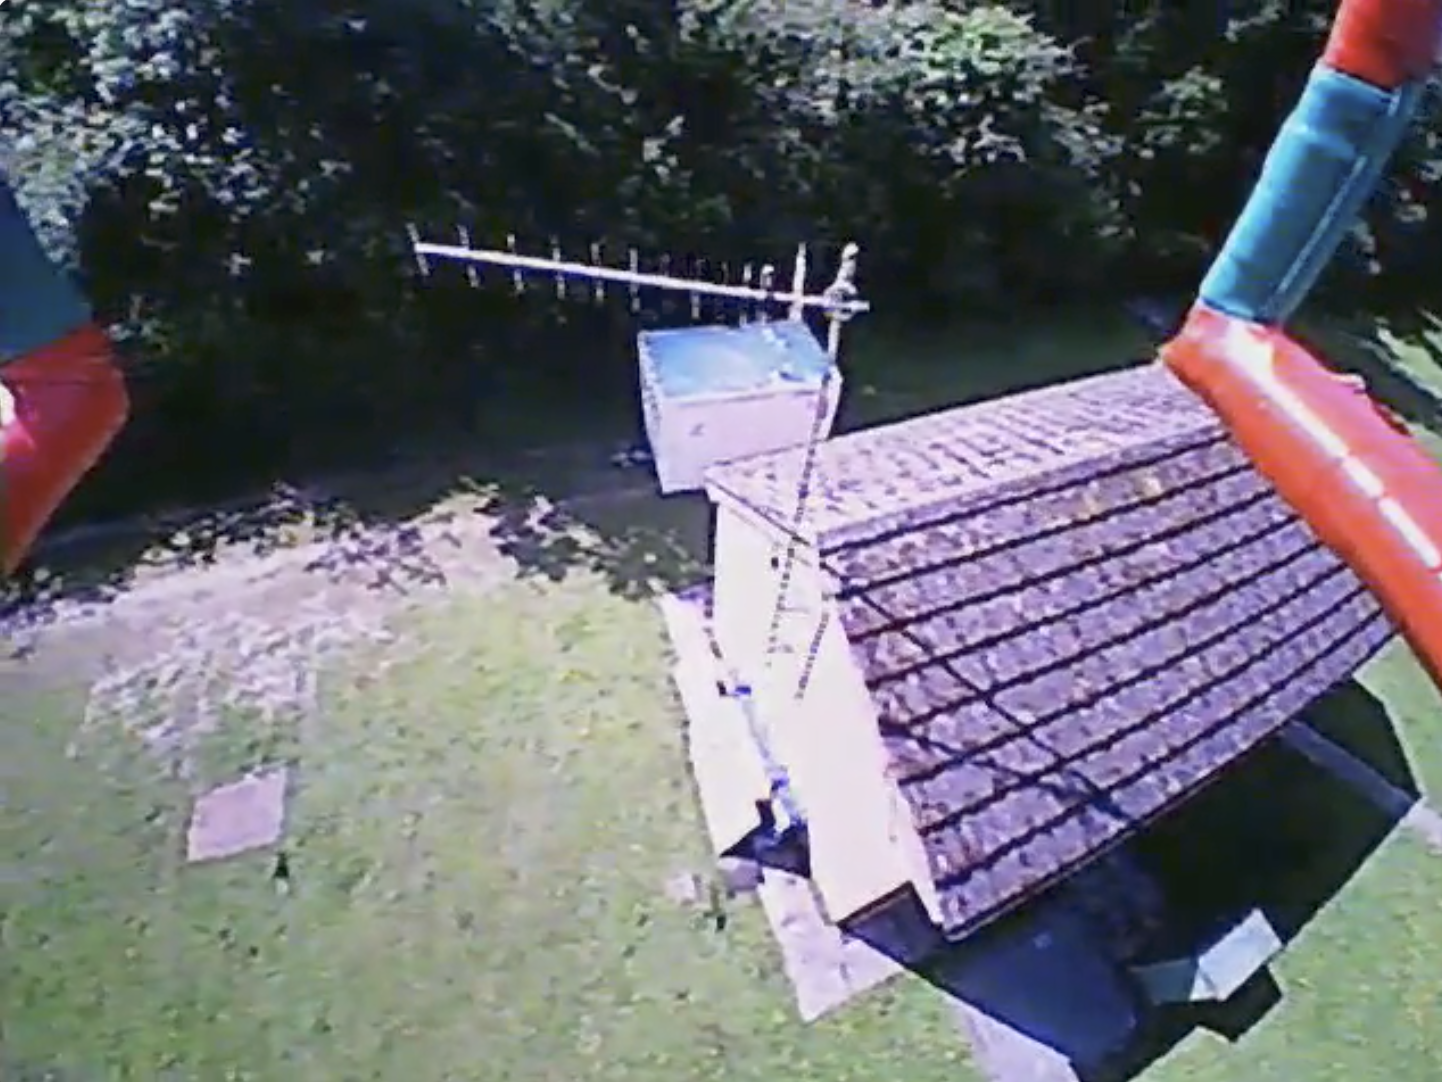
\includegraphics[width=\columnwidth]{Figures/radio_antenna_inspection.png}
    \caption{A screen capture of the live feed coming from the UAV, performing a visual inspection of a radio antenna installed in a location that is difficult and for personnel to access.}
    \label{fig:radio_antenna_inspection}
\end{figure}

\begin{figure}[h]
    \centering
    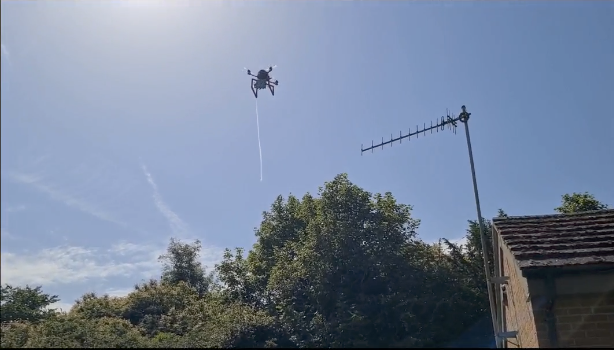
\includegraphics[width=\columnwidth]{Figures/Drone_Capturing_Footage.png}
    \caption{The UAV in flight while autonomously capturing visual inspection data. The onboard camera system enables the inspection of infrastructure from multiple viewpoints while maintaining a safe distance from the asset.}
    \label{fig:drone_capturing_footage}
\end{figure}

\section{Conclusion}

This project demonstrated the successful design, assembly, calibration and testing of an ArduPilot-based quadcopter. The final UAV combined a 3D-printed frame, MicoAir flight controller, GPS/compass module, ExpressLRS receiver, telemetry system, FPV camera and Lua-based autonomous flight control.

The main takeaway was that reliable drone performance depends on the integration of mechanical design, wiring, software configuration, sensor calibration and safe testing procedures. Several issues, including radio setup, compass detection, flight-controller failure and software compatibility, required systematic troubleshooting before the drone could operate correctly.

The camera and computer-vision elements also showed how a low-cost UAV could be adapted for practical inspection tasks, particularly in hazardous or difficult-to-access environments. Future improvements would focus on better component protection, a more durable design, GPS-independent navigation, camera stabilisation, and more extensive physical flight testing.

\begin{thebibliography}{99}

\bibitem{micoair743}
MicoAir Tech,
\textit{MicoAir743 V2 AIO 45A Flight Controller}.
Available: \url{https://micoair.com/flightcontroller_micoair743v2_aio_45a/}

\bibitem{missionplanner}
ArduPilot,
\textit{Installing Mission Planner}.
Available: \url{https://ardupilot.org/planner/docs/mission-planner-installation.html}

\bibitem{heliguy}
Heliguy,
\textit{Heliguy Pre-Flight Checklist}.
Available: \url{https://www.heliguy.com/blogs/posts/heliguy-pre-flight-checklist/}

\bibitem{lua}
Wikipedia,
\textit{Lua}.
Available: \url{https://en.wikipedia.org/wiki/Lua}

\bibitem{eeops}
O. Vogt,
\textit{Continuous Professional Development by Exploring Entrepreneurial Opportunities Using Drones (EEOPS-D)}.
Presentation, Durham University, Department of Engineering, 2026.

\end{thebibliography}\textbf{}


\section*{AI Disclaimer}

Artificial Intelligence (Grammarly, ChatGPT) was used to help improve the readability and structure of this document.
\onecolumn

%=================================================
% APPENDIX
% =================================================

\appendices


\section*{Additional Troubleshooting Evidence}
\label{app:troubleshooting}

\begin{table*}[htbp]
\caption{Autonomous Flight Development and Troubleshooting Summary}
\label{tab:lua-troubleshooting}
\centering
\footnotesize
\renewcommand{\arraystretch}{1.15}
\begin{tabularx}{\textwidth}
{@{}
p{0.18\textwidth}
p{0.21\textwidth}
p{0.25\textwidth}
X
@{}}
\toprule
\textbf{Issue} &
\textbf{Cause} &
\textbf{Resolution} &
\textbf{Engineering significance} \\
\midrule

SITL failed to launch &
Required Cygwin DLL dependencies were absent from the active SITL directory &
Restored the required runtime files beside \texttt{ArduCopter.exe} &
Demonstrated that dependency-management faults can prevent execution
independently of the flight-control algorithm \\

DLL repair initially failed &
OneDrive redirected the active Mission Planner Documents and SITL path &
Located and modified the actual Mission Planner SITL working directory &
Confirmed that path consistency and identification of the active executable
directory are critical \\

Lua operation required verification &
A later navigation failure could otherwise have originated from the script
directory, interpreter, scheduler or telemetry link &
Ran a minimal diagnostic script and confirmed repeated
\texttt{LUA\_TEST} messages &
Separated the scripting environment from later navigation-code faults \\

Scripting pre-arm error &
Unsupported \texttt{set\_alt\_m()} Lua API call &
Replaced the command with firmware-compatible altitude functions and separate
reference-frame handling &
Demonstrated dependence between the Lua API and the installed ArduPilot
firmware version \\

Script could activate unexpectedly &
The auxiliary scripting switch could already be HIGH when the script
initialised &
Required a deliberate LOW-to-HIGH transition after startup &
Reduced the risk of unintended autonomous activation immediately after boot \\

Vehicle would not re-arm &
The previous flight left the vehicle in LAND mode &
Selected STABILIZE before arming and then reactivated
\texttt{Scripting1} &
Confirmed operation of the normal ArduPilot mode-dependent arming safety
interlock \\

LOITER caused descent &
The simulated throttle input was not centred &
Used BRAKE for pilot-override testing &
Showed that different flight modes retain different dependencies on pilot
inputs \\

Pilot override required verification &
The script could otherwise continue issuing GUIDED position commands &
Detected external mode changes and terminated scripted navigation commands &
Confirmed that manual and failsafe control retained priority over the Lua
mission \\

Return error appeared large &
The final target was accepted once the vehicle entered the
$0.8\,\mathrm{m}$ radius &
Added direct error reporting and repeated the desktop test six times &
Replaced subjective judgement with repeatable quantitative validation \\

Simulation screenshot differed from the main dataset &
The screenshot was obtained later using a separate laptop SITL installation and
firmware build &
Reported it as an illustrative run and excluded its $0.78\,\mathrm{m}$ result
from the six-trial dataset &
Preserved traceability between visual evidence and the quantitative results \\
\bottomrule
\end{tabularx}
\end{table*}

\end{document}
